\begin{multicols*}{2}

    \chapter{Gestión Operativa con Entornos de Orquestación y Enfoque SRE}
Al desplegar una LLM (Large Language Model) con Podman, rápidamente me di cuenta de las limitaciones de una orquestación manual. Aunque Podman es excelente para la gestión de contenedores individuales, surgieron desafíos significativos al pensar en el entorno de producción. ¿Cómo podría monitorizar el rendimiento de la LLM a alto nivel, similar a lo que ofrece Grafana? Gestionar que la aplicación se adaptará a las variaciones de carga y que se mantuviera funcionando sin interrupciones se volvía una tarea compleja y propensa a errores. Además, la gestión de los logs de múltiples contenedores resultaba poco intuitiva y demandaba un esfuerzo considerable. Todas estas dificultades dejaron claro que necesitamos herramientas y estrategias que automaticen y simplifiquen estas tareas, algo fundamental para que los sistemas sean eficientes y robustos en un entorno SRE.

     En este contexto, se descubrió OpenShift, una plataforma integrada que agrupa capacidades como el escalado automático, la recuperación ante fallos, la gestión avanzada de logs y la monitorización unificada. Desde la perspectiva de SRE, OpenShift facilita la implementación de buenas prácticas desde el diseño hasta la operación, siguiendo recomendaciones sobre diseño resiliente y seguridad integrada.

     Además, la Universidad de Granada (UGR) ofreció la oportunidad de realizar un curso específico de OpenShift DO180. Aprovechando esta formación, este trabajo complementa la teoría mostrando la utilidad de OpenShift para automatizar despliegues, mejorar la observabilidad y gestionar servicios de manera eficiente.

     En este ámbito, el concepto de LLMOps es especialmente relevante. LLMOps abarca el conjunto de prácticas, herramientas y procesos para la operación eficiente de modelos de lenguaje a gran escala, incluyendo despliegue, monitorización, escalado y mantenimiento continuo en producción. Integrar prácticas de LLMOps en proyectos basados en OpenShift es un avance natural para mejorar la gestión, asegurar la escalabilidad y reducir el esfuerzo manual en la operación diaria de los modelos.


\vspace{\baselineskip}

\section{Introducción a OpenShift}

OpenShift es una plataforma que permite a las organizaciones desplegar aplicaciones en contenedores de manera eficiente y escalable. Construida sobre Kubernetes, añade una capa de abstracción y automatización que simplifica tareas esenciales del ciclo de vida de las aplicaciones, adaptándose a diversos entornos (desarrollo, pruebas, producción).

La importancia de OpenShift radica en su capacidad para gestionar aplicaciones en contenedores de forma declarativa. Los administradores definen el estado deseado de las aplicaciones (mediante archivos YAML o JSON), y la plataforma se encarga automáticamente de mantenerlo, ajustándose a cambios o imprevistos. Esta característica reduce la carga operativa, aporta consistencia y su integración con herramientas de observabilidad y flujos de trabajo de desarrollo la hace atractiva para entornos empresariales que buscan agilidad y confiabilidad.

En cuanto a su funcionamiento, OpenShift utiliza contenedores para empaquetar aplicaciones y sus dependencias, ofreciendo aislamiento respecto al sistema operativo del host. A diferencia de las máquinas virtuales, los contenedores comparten el kernel subyacente y operan en espacios aislados (namespaces), lo que disminuye la carga del sistema y mejora la portabilidad de las aplicaciones.

\begin{figure}[H]
    \centering
    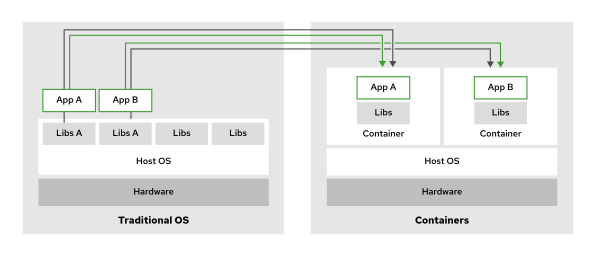
\includegraphics[width=\linewidth]{imagenes/image37.png}
    \caption{Aplicaciones en contenedores frente al sistema operativo del host}
    \label{fig:server2}
\end{figure}

\subsection{Tipos de instalación}

OpenShift ofrece varias opciones de instalación, adaptadas a las necesidades específicas de cada usuario, desde entornos de desarrollo hasta implementaciones de producción a gran escala.

\vspace{\baselineskip}

\noindent\textbf{OpenShift Local:} 
OpenShift Local permite implementar un clúster de OpenShift directamente en una computadora personal. Es ideal para pruebas, desarrollo y exploración inicial de la plataforma, proporcionando un entorno rápido y fácil de configurar. Su propósito principal es servir como espacio de familiarización y experimentación, no para entornos de producción. Esta es la opción seleccionada para este trabajo, permitiendo seguir utilizando el servidor para demostrar las capacidades de OpenShift.

\vspace{\baselineskip}

\noindent\textbf{Sandbox para desarrolladores:} 
Para quienes desean probar OpenShift sin costos iniciales, Red Hat ofrece el Sandbox para Desarrolladores. Este servicio proporciona acceso gratuito durante 30 días a un clúster de OpenShift compartido, útil para familiarizarse con la plataforma y realizar pruebas en un entorno controlado. Sin embargo, su naturaleza temporal y compartida lo hace inadecuado para implementaciones de producción.

\vspace{\baselineskip}

\noindent\textbf{Ediciones gestionadas de Red Hat OpenShift:} 
Las organizaciones que buscan soluciones de producción con menor carga operativa pueden optar por las Ediciones gestionadas de Red Hat OpenShift. Estas incluyen servicios en la nube administrados por Red Hat y proveedores asociados (ej. Red Hat OpenShift Service on AWS, Azure Red Hat OpenShift). En estas ediciones, Red Hat y el proveedor se encargan de la gestión, mantenimiento y actualizaciones del clúster, lo que reduce significativamente las responsabilidades del usuario, aunque puede implicar ciertas limitaciones (ej. menor control sobre la autenticación).


\subsection{Arquitectura y Componentes de OpenShift}

OpenShift se basa en la arquitectura modular de Kubernetes, extendiendo sus funcionalidades para ofrecer una plataforma robusta en la gestión de aplicaciones en contenedores. Esta combinación aprovecha la escalabilidad y tolerancia a fallos de Kubernetes, a la vez que introduce capacidades adicionales de automatización y control propias de OpenShift.

\begin{figure}[H]
    \centering
    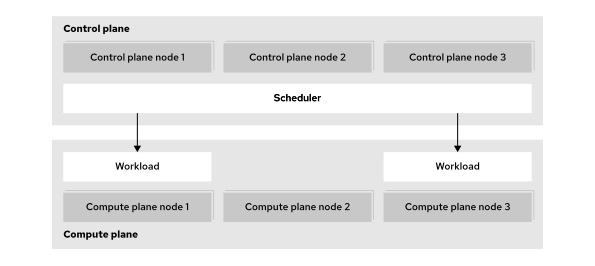
\includegraphics[width=\linewidth]{imagenes/image38.png}
    \caption{Componentes de Kubernetes}
    \label{fig:k8s-components}
\end{figure}

\subsubsection*{Componentes Fundamentales de Kubernetes}
La arquitectura de OpenShift se fundamenta en los componentes esenciales de Kubernetes. Los nodos del plano de control coordinan globalmente el clúster, gestionando la programación de cargas de trabajo y manteniendo el estado del sistema mediante servicios como la API de Kubernetes, el scheduler y el controller manager. Por su parte, los nodos del plano de cómputo ejecutan las cargas de trabajo del usuario, alojando los pods con las aplicaciones en contenedores. Esta separación mejora la estabilidad y seguridad, previniendo interferencias y reforzando la escalabilidad y tolerancia a fallos.

La API de Kubernetes, enriquecida en OpenShift con recursos personalizados, permite definir las cargas de trabajo mediante un modelo de configuración declarativa. Los usuarios especifican el estado deseado de las aplicaciones a través de archivos YAML o JSON, y OpenShift se encarga de mantenerlo automáticamente. Este enfoque sigue un ciclo de "Definir → Aplicar → Monitorizar → Ajustar", lo que reduce errores manuales y simplifica la gestión a gran escala. Además, los espacios de nombres (namespaces) son cruciales para organizar y aislar recursos dentro del clúster, facilitando la gestión granular de permisos y el control de acceso en entornos multi-equipo o multi-proyecto.

\begin{figure}[H]
    \centering
    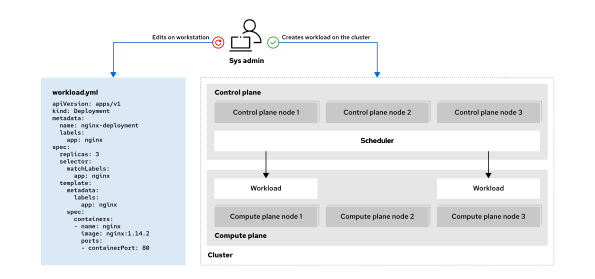
\includegraphics[width=\linewidth]{imagenes/image39.png}
    \caption{Gestión de recursos declarativa}
    \label{fig:declarative-management}
\end{figure}

\subsubsection*{Extensiones específicas de OpenShift}
OpenShift amplía las capacidades de Kubernetes con herramientas diseñadas para optimizar el flujo de trabajo de desarrollo y operaciones. Su entorno integrado para desarrolladores simplifica el ciclo de vida de las aplicaciones.

El registro de contenedores incorporado permite almacenar y gestionar imágenes de forma nativa, eliminando la necesidad de soluciones externas y mejorando la seguridad. Para automatizar procesos, OpenShift incluye pipelines de CI/CD listos para usar, que facilitan la integración y entrega continua con mínima intervención manual.

Otra herramienta poderosa es Source-to-Image (S2I), que crea imágenes de contenedores directamente desde el código fuente en repositorios como Git. Esto agiliza la construcción y estandariza las imágenes, reduciendo errores y aumentando la eficiencia del desarrollo.

En cuanto a observabilidad, OpenShift ofrece un conjunto completo de herramientas para monitorear aplicaciones e infraestructura. Los equipos pueden acceder a métricas en tiempo real, configurar alertas proactivas y analizar registros desde la consola web integrada. Esta visibilidad es crucial para mantener la confiabilidad y el rendimiento de las aplicaciones en producción, permitiendo detectar y resolver problemas de forma proactiva.

\subsection{OpenShift y SRE}

Una de las cualidades más destacadas de OpenShift es su capacidad para facilitar la implementación de prácticas SRE, al añadir un entorno robusto y flexible a Kubernetes.

\noindent\textbf{Automatización y escalabilidad:}  
OpenShift incorpora mecanismos avanzados como el autoescalado horizontal (HPA) y operadores para gestionar recursos dinámicamente. Esto permite que las aplicaciones se adapten automáticamente a fluctuaciones en la demanda sin intervención manual constante. La plataforma automatiza tareas operativas críticas como el aprovisionamiento de recursos y el balanceo de carga, reduciendo errores humanos y manteniendo la estabilidad del sistema bajo cargas variables.

\noindent\textbf{Observabilidad proactiva:}  
La plataforma integra soluciones como Prometheus para recolección de métricas y Grafana para visualización, proporcionando una visión completa y en tiempo real del estado del clúster y las aplicaciones. Esta capacidad permite monitorear el rendimiento actual y establecer alertas predictivas. Los equipos pueden detectar anomalías tempranamente, investigar incidentes mediante análisis forenses detallados y realizar mejoras continuas basadas en datos concretos.

\noindent\textbf{Gestión del ciclo de vida con CI/CD:}  
OpenShift simplifica los flujos de trabajo de integración y despliegue continuo mediante herramientas como Jenkins y Tekton. La plataforma soporta estrategias avanzadas de despliegue (ej. rolling updates, despliegues azul-verde), permitiendo implementar cambios con mínimo riesgo. En caso de problemas, los rollbacks automatizados garantizan una rápida recuperación. Todo esto facilita el equilibrio entre velocidad de entrega y estabilidad operacional.

\noindent\textbf{Resiliencia y seguridad integrada:}  
La arquitectura de OpenShift está diseñada para alta disponibilidad, con características como replicación automática de pods y distribución inteligente de cargas de trabajo. Las Security Context Constraints (SCC) implementan el principio de mínimo privilegio, mientras que el cifrado de datos en tránsito y en reposo protege la información sensible. El control de acceso granular mediante RBAC (Role-Based Access Control) asegura que solo usuarios autorizados realicen cambios críticos en el sistema.

\end{multicols*}

\begin{figure}[H]
    \centering
    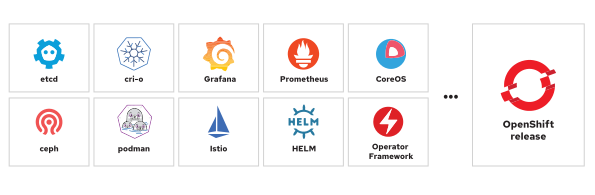
\includegraphics[width=0.85\linewidth]{imagenes/image40.png}
    \caption{Proyectos de código abierto en una versión de OpenShift}
    \label{fig:openshift-ecosystem}
\end{figure}
\noindent\textit{La integración con el ecosistema CNCF (Cloud Native Computing Foundation) asegura interoperabilidad y flexibilidad.}

\vspace{\baselineskip}
%tutorial


\section{Despliegue y administración de aplicaciones}

Esta sección detalla el proceso de despliegue y gestión de una aplicación full-stack en OpenShift. En la demostración se realiza sobre el entorno OpenShift Sandbox proporcionado por Red Hat, ya que la virtualización de OpenShift Local impidió la conexión con la GPU del servidor y las limitaciones del port forwarding (posiblemente por la gestión de dos saltos de conexión) obstaculizaron el acceso a la interfaz web. Este entorno simulará un ecosistema de producción con el fin de demostrar y validar los principios fundamentales de Site Reliability Engineering (SRE). Este enfoque permite ilustrar el uso de herramientas nativas de orquestación, aprovisionamiento, observabilidad y fiabilidad, reflejando un caso de uso realista alineado con las prácticas de Site Reliability Engineering (SRE).

Para la demostración, se utilizará la interfaz de línea de comandos (CLI) de OpenShift (\texttt{oc}), lo que garantiza la reproducibilidad de los pasos. Aunque OpenShift ofrece una potente interfaz web, todas las acciones realizadas mediante la CLI tienen su equivalente gráfico. Se utilizará para la demostración como base los tutoriales y ejemplos disponibles del repositorio \url{https://github.com/sclorg/}, que también se usan en el curso Openshift DO180 realizado.

Una recomendación a la hora de manejar la terminal es configurar alias para las cuentas de administrador y desarrollador:

\footnotesize
\begin{verbatim}
$ echo "alias al='oc login -u admin -p redhatocp https://api.ocp4.example.com:6443'"\
 >> ~/.bashrc

$ echo "alias dl='/usr/local/bin/oc login -u developer\
 -p developer https://api.ocp4.example.com:6443'" >> ~/.bashrc

$ source ~/.bashrc
\end{verbatim}

Para saber la URL de la consola web asociada a la sesión de OpenShift:
\begin{verbatim}
$ oc whoami --show-console
\end{verbatim}

Con una sesión de developer (usando el alias \texttt{dl}) es suficiente para esta demostración.

\vspace{\baselineskip}

\subsection{Source-to-Image (S2I)}

Me gustaría comenzar hablando más a fondo sobre Source-to-Image (S2I), una herramienta robusta que simplifica la creación de imágenes de contenedores reproducibles directamente desde el código fuente de una aplicación. Su propósito principal es permitir a los desarrolladores transformar su código en una imagen ejecutable de forma sencilla y eficiente, integrando el código con una imagen base ("builder image") que contiene el entorno de construcción y ejecución.

El flujo de trabajo de S2I implica la inyección del código fuente y scripts personalizados (como \texttt{assemble} y \texttt{run}) dentro de un contenedor basado en la imagen del constructor. El script \texttt{assemble} se encarga de compilar, instalar dependencias y preparar la aplicación, mientras que el script \texttt{run} la inicia. El resultado es una nueva imagen de contenedor lista para desplegar.

Generalmente, para que S2I interactúe correctamente con el código fuente, es necesario definir explícitamente scripts como \texttt{assemble}, \texttt{run}, \texttt{save-artifacts}, etc., que residen en el directorio \texttt{.s2i/bin/} del repositorio. Sin embargo, en el caso de aplicaciones Node.js estándar, como la que se encuentra en el repositorio que usamos, OpenShift sabe cómo manejar este tipo de aplicaciones internamente sin necesidad de añadir scripts personalizados al repositorio. Toma el código fuente, instala automáticamente las dependencias (\texttt{npm install}), y luego ejecuta la aplicación.

\begin{figure}[H]
    \centering
    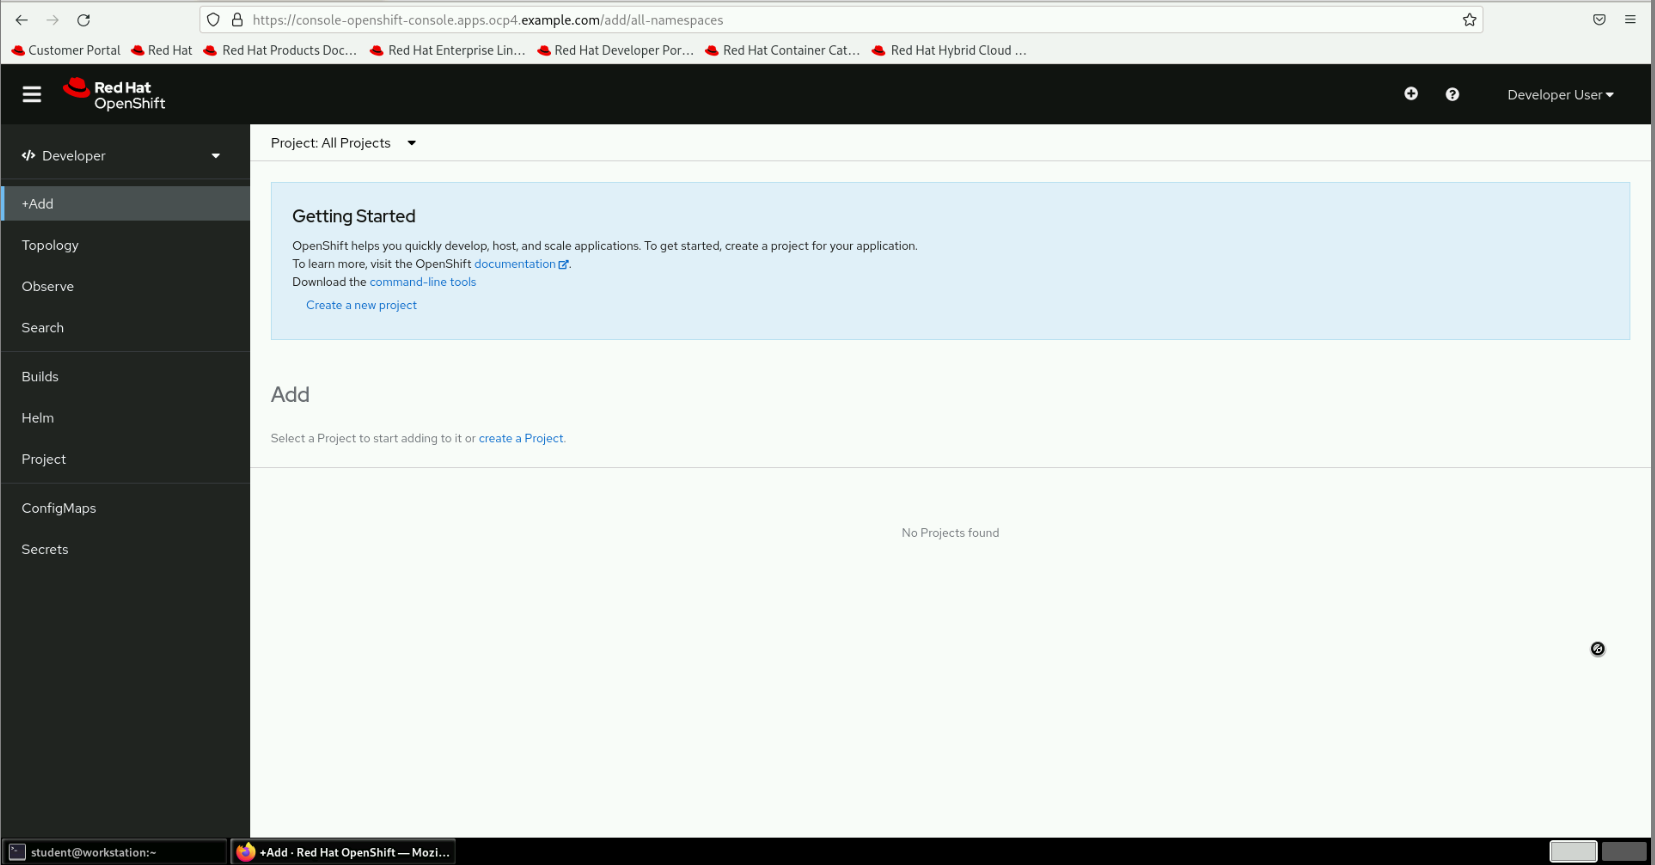
\includegraphics[width=1\linewidth]{imagenes/image4.png}
    \caption{Proceso de Source-to-Image (S2I)}
    \label{fig:openshift-ecosystem}
\end{figure}


\subsection{Creación del proyecto de trabajo}

Para aislar todos los recursos de la demostración y mantenerlos organizados, se creó un nuevo proyecto en OpenShift:
\begin{verbatim}
oc new-project sre-demo
\end{verbatim}

\subsection{Despliegue del frontend desde GitHub}

Se utilizó la aplicación de ejemplo \texttt{nodejs-ex} del repositorio de Red Hat, que contiene una interfaz web básica para la gestión de frutas. Dicho despliegue se realizó con el comando \texttt{oc new-app}, que, como se explicó previamente, utiliza la funcionalidad Source-to-Image (S2I):

\begin{verbatim}
oc new-app https://github.com/sclorg/nodejs-ex --name=nodejs-ex
\end{verbatim}

OpenShift detecta el tipo de aplicación (Node.js en este caso) y automáticamente crea y configura los objetos necesarios para su despliegue y gestión: un \texttt{BuildConfig}, un \texttt{DeploymentConfig} (o \texttt{Deployment} en versiones recientes de OpenShift) y un \texttt{Service}. En la vista de topología de la consola web, el pod aparecerá con un color naranja, indicando que se está creando o construyendo.

\begin{figure}[H]
    \centering
    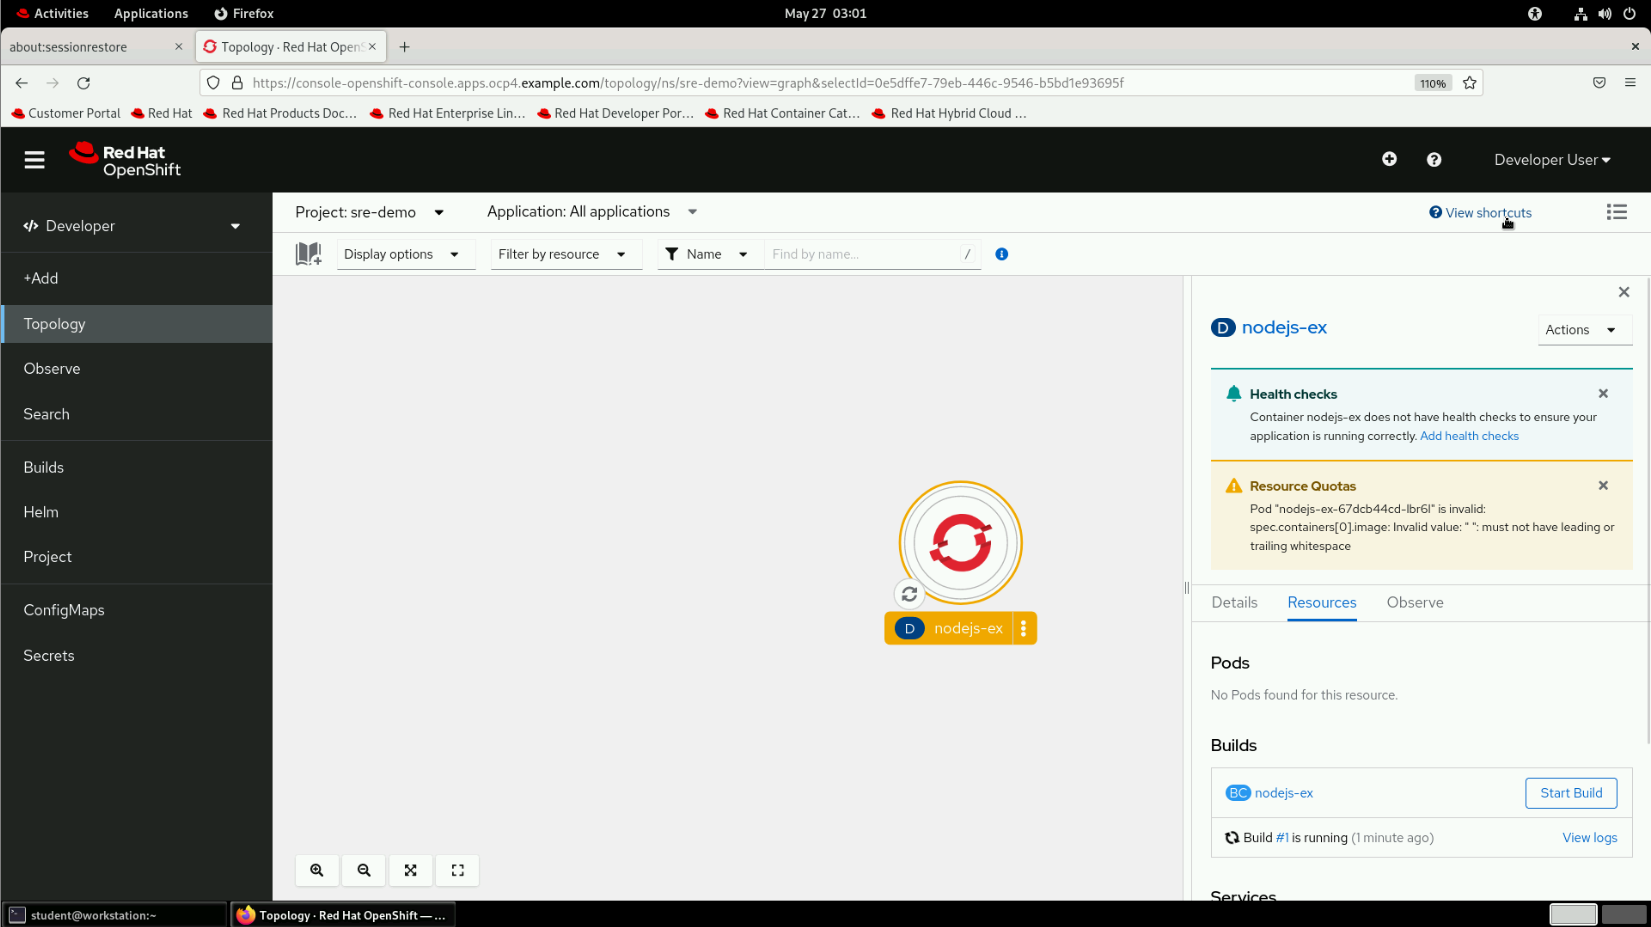
\includegraphics[width=1\linewidth]{imagenes/image11.png}
    \caption{Proceso de Source-to-Image (S2I)}
    \label{fig:openshift-ecosystem}
\end{figure}

Ahora necesitamos exponer este servicio públicamente. Con \texttt{oc expose} se genera una URL pública para acceder a la aplicación:

\begin{verbatim}
oc expose service nodejs-ex
\end{verbatim}

\begin{figure}[H]
    \centering
    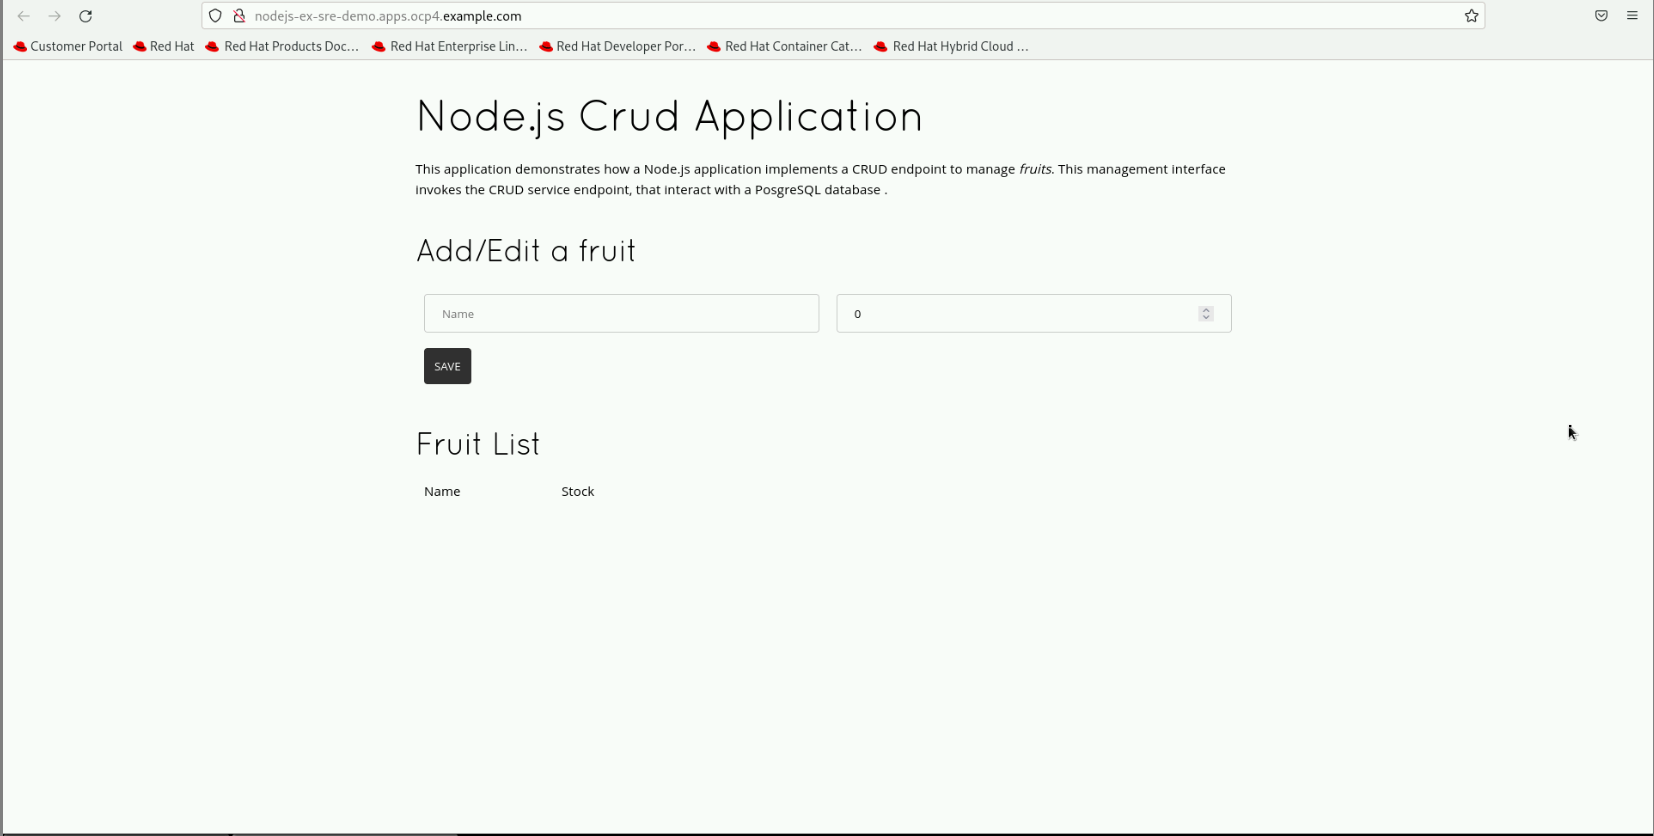
\includegraphics[width=1\linewidth]{imagenes/image9.png}
    \caption{Proceso de Source-to-Image (S2I)}
    \label{fig:openshift-ecosystem}
\end{figure}

\vspace{\baselineskip}

\subsection{Verificación y Diagnóstico del Frontend}

Al intentar interactuar con la aplicación desplegada a través de la URL generada, se desplegó la aplicación pero no podíamos realizar acciones CRUD. En principio, deberíamos ser capaces de añadir frutas a una lista, por lo que tenemos que diagnosticar el problema. Primero, se obtuvieron los pods del proyecto:
\begin{verbatim}
oc get pods
\end{verbatim}

Luego, se consultaron los logs de la instancia del pod del frontend:
\begin{verbatim}
oc logs nodejs-ex-6d6c6d6b79-ckxb8
\end{verbatim}

Los logs revelaron el siguiente error:
\begin{verbatim}
{"level":50,"time":1747902770555,"pid":21,"hostname":"nodejs-ex-6d6c6d6b79-ckxb8","err":\
{"type":"Error","message":"connect ECONNREFUSED <IP_DEL_BACKEND>:5432","stack":\
"Error: connect ECONNREFUSED <IP_DEL_BACKEND>:5432\n	at TCPConnectWrap.afterConnect \
[as oncomplete] (node:net:1607:16)","errno":-111,"code":"ECONNREFUSED","syscall":"connect"\
,"address":"<IP_DEL_BACKEND>","port":5432},"msg":"connect ECONNREFUSED <IP_DEL_BACKEND>:5432"}
\end{verbatim}

Este mensaje de \texttt{ECONNREFUSED} nos confirmó que la aplicación intenta conectarse a una base de datos PostgreSQL, que aún no estaba desplegada.




\section{Gestión de almacenamiento y configuración externa}

\subsection{Despliegue de PostgreSQL}

Para proporcionar el backend de datos, se desplegó una instancia persistente de PostgreSQL. La persistencia es crucial para que los datos de la base de datos no se pierdan si el pod se reinicia o se mueve a otro nodo. Se utilizó el siguiente comando para desplegar PostgreSQL, configurando las credenciales de usuario y la base de datos:
\begin{verbatim}
oc new-app postgresql-persistent -p POSTGRESQL_USER=user -p POSTGRESQL_PASSWORD=password\
 -p POSTGRESQL_DATABASE=nodejsdb --name=postgresql
\end{verbatim}

Este comando automatiza la creación de varios objetos clave en OpenShift: un DeploymentConfig (para gestionar el despliegue del pod de PostgreSQL), un Service denominado \texttt{postgresql} (que permite al frontend conectarse a la base de datos), un PersistentVolumeClaim (PVC) de 1Gi para la persistencia de datos, y un Secret que almacena de forma segura las credenciales.

El PersistentVolumeClaim (PVC) es una solicitud de almacenamiento por parte de la aplicación. Actúa como una abstracción que permite al pod de PostgreSQL solicitar y consumir almacenamiento persistente sin necesidad de conocer los detalles específicos de la infraestructura subyacente. OpenShift se encarga de enlazar este PVC con un PersistentVolume (un recurso de almacenamiento provisionado en el clúster) que cumpla con los requisitos del PVC, asegurando así que los datos de la base de datos no se pierdan entre reinicios o movimientos del pod. Se verifica la creación del PVC con:
\begin{verbatim}
oc get pvc
\end{verbatim}

El resultado esperado muestra el PVC en estado Bound, lo que indica la asignación exitosa de un volumen:
\begin{verbatim}
NAME        STATUS   VOLUME                              CAPACITY   ACCESS   STORAGECLASS   AGE
postgresql  Bound    pvc-8ec339dc-0fe3-4f7b-b13f-0ee6   1Gi       RWO      gp3           38s
\end{verbatim}


\begin{figure}[H]
    \centering
    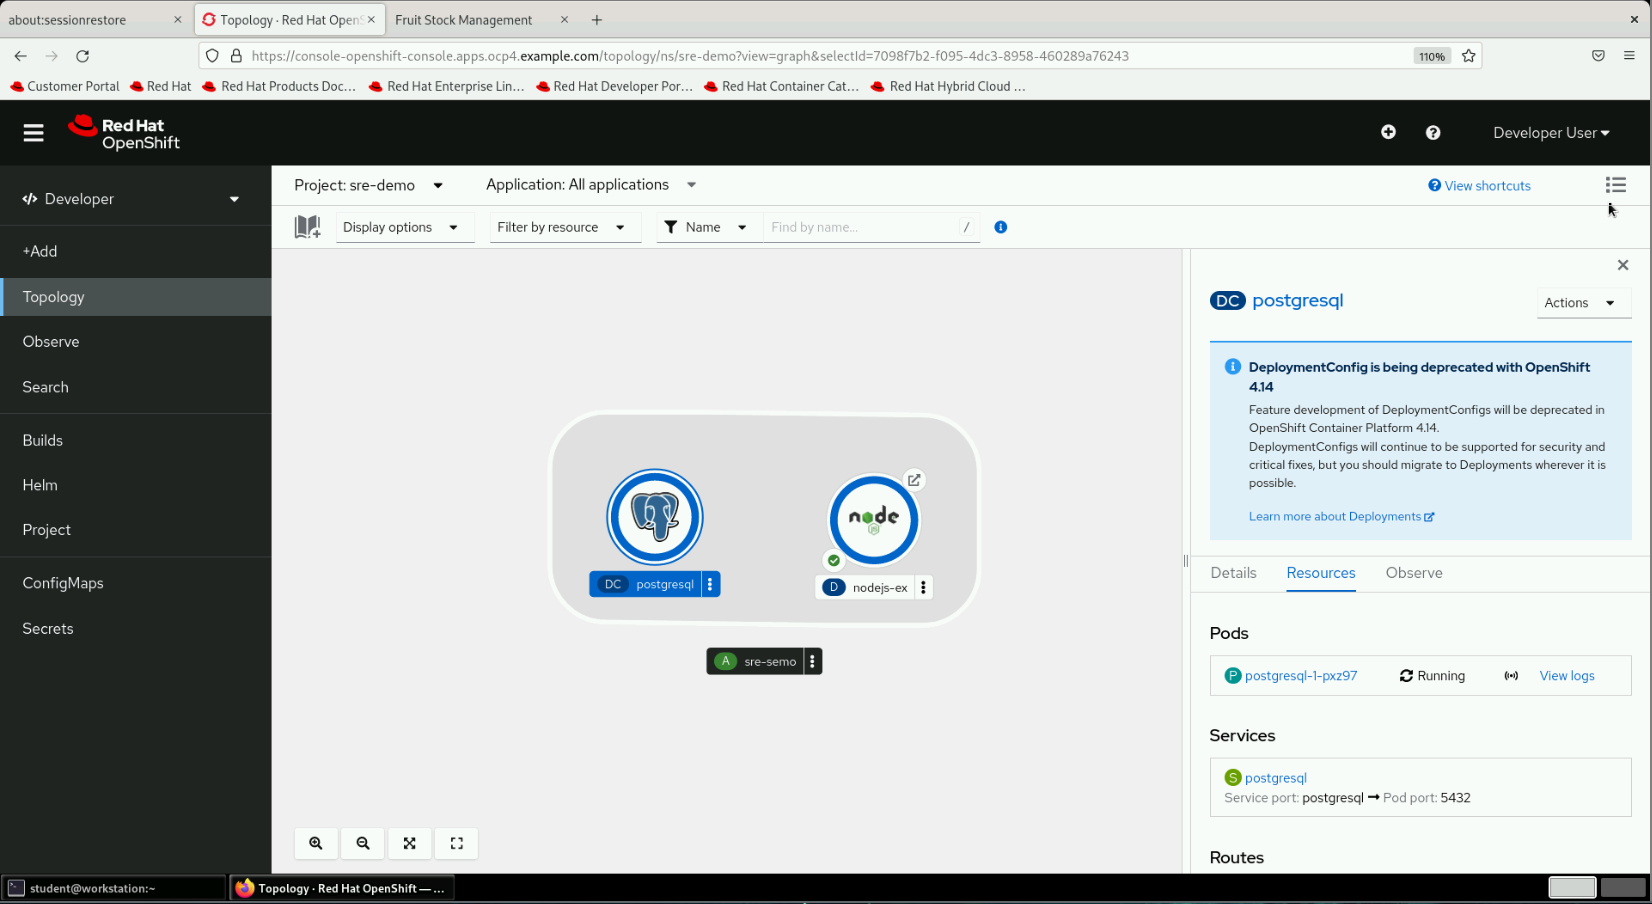
\includegraphics[width=0.95\linewidth]{imagenes/image88.png}
    \caption{Proceso de Source-to-Image (S2I)}
    \label{fig:openshift-ecosystem}
\end{figure}

Desde la interfaz web de OpenShift, se puede crear una aplicación para englobar estos pods, lo que mejora la visualización en la vista de topología. Incluso se pueden añadir etiquetas a los deployments (ej. \texttt{app.kubernetes.io/name=postgresql}, \texttt{app.kubernetes.io/name=nodejs}) para cambiar los iconos y hacerlos más visuales y organizados en la interfaz.


\subsection{Conexión del Frontend con el Backend}

Una vez que el servicio de PostgreSQL estuvo disponible y su almacenamiento configurado, se establecieron las variables de entorno en el deployment del frontend (\texttt{nodejs-ex}) para que pudiera conectarse a la base de datos recién desplegada:
\begin{verbatim}
oc set env deployment/nodejs-ex POSTGRESQL_USER=user POSTGRESQL_PASSWORD=password\
 POSTGRESQL_DATABASE=nodejsdb DATABASE_SERVICE_NAME=postgresql
\end{verbatim}

Para que el frontend aplicara estos cambios y reiniciara con las nuevas variables de entorno, se ejecutó un rollout restart:
\begin{verbatim}
oc rollout restart deployment/nodejs-ex
\end{verbatim}

Tras este paso, la aplicación del frontend comenzó a funcionar correctamente, sin el error previo de conexión a la base de datos, integrando backend con frontend. La vista de topología mostrará ahora la conexión entre el frontend y el backend.

\begin{figure}[H]
    \centering
    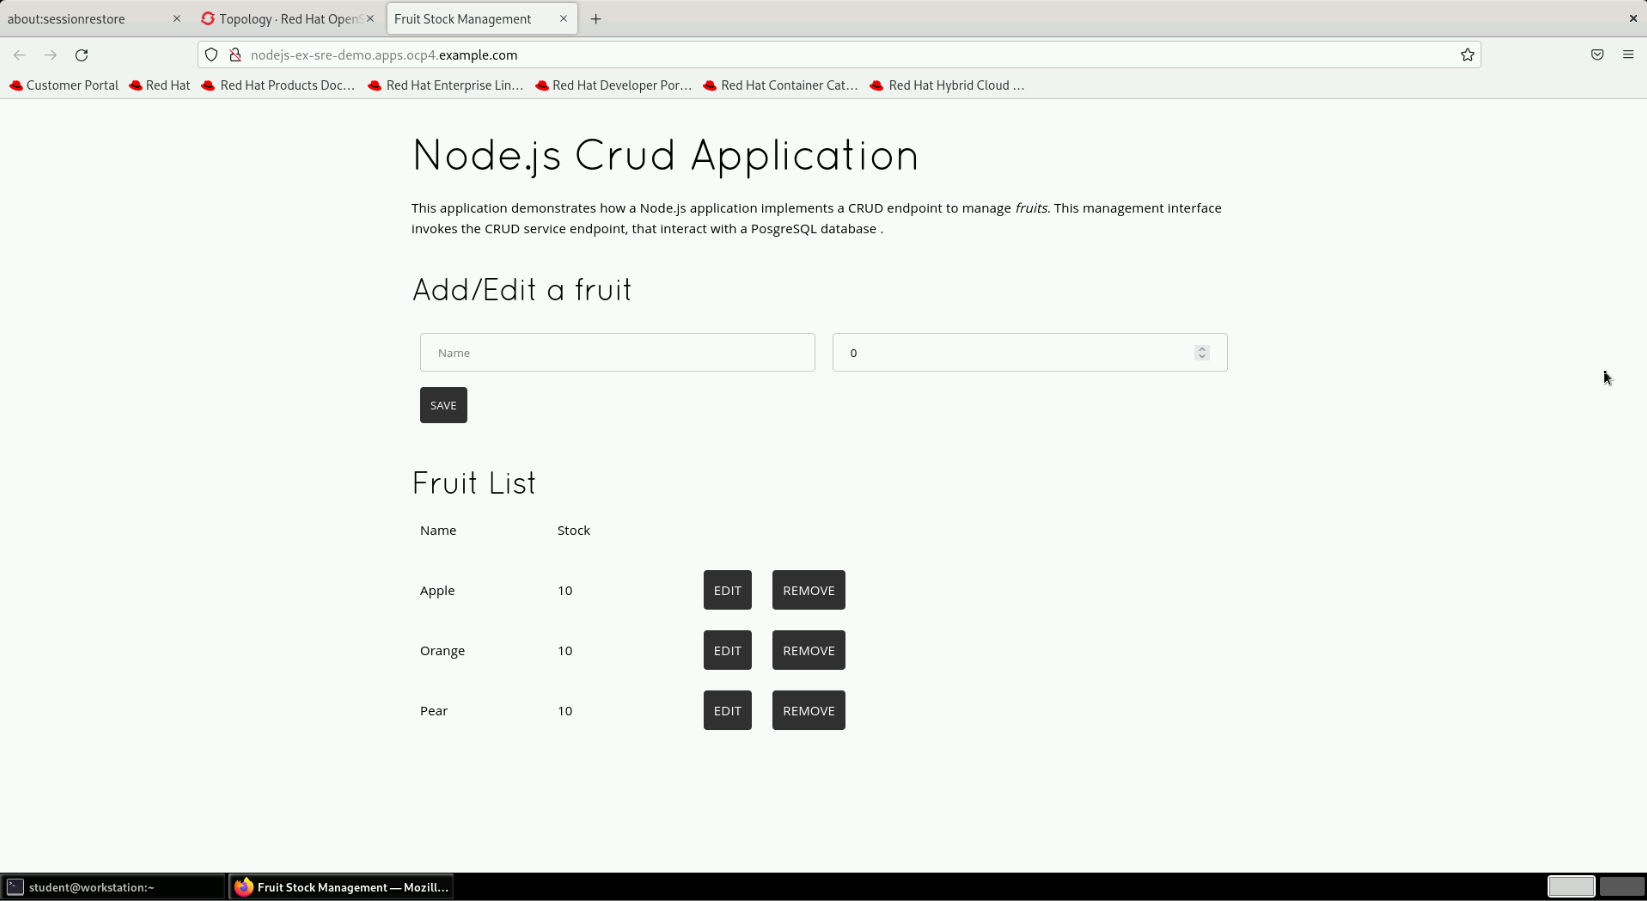
\includegraphics[width=1\linewidth]{imagenes/image12.png}
    \caption{Proceso de Source-to-Image (S2I)}
    \label{fig:openshift-ecosystem}
\end{figure}

\newpage

\section{Monitorización de cargas de trabajo}

OpenShift ofrece diversas herramientas para la monitorización, que van desde la línea de comandos hasta una consola web avanzada, importantes para la observabilidad en un entorno SRE.

\subsection{Uso de herramientas básicas desde CLI}

Para una monitorización rápida y básica del uso de recursos de pods y nodos, se emplean los siguientes comandos, que proporcionan una visión general del rendimiento del clúster:
\begin{verbatim}
oc adm top pods
oc adm top nodes
\end{verbatim}

\subsection{Monitorización avanzada (web)}

La consola web de OpenShift proporciona herramientas de observabilidad más completas, permitiendo un análisis detallado del estado de la infraestructura y las aplicaciones:

\begin{itemize}
    \item \textbf{Observe → Dashboards:} Ofrece visualizaciones gráficas de métricas clave como CPU, memoria y estado de los pods.
    \item \textbf{Observe → Metrics:} Permite realizar consultas PromQL personalizadas para un análisis al igual que Grafana.
\end{itemize}

Estas capacidades son fundamentales para establecer umbrales de alerta, configurar notificaciones proactivas y tomar decisiones informadas sobre el escalado o los ajustes de recursos.

\begin{figure}[H]
    \centering
    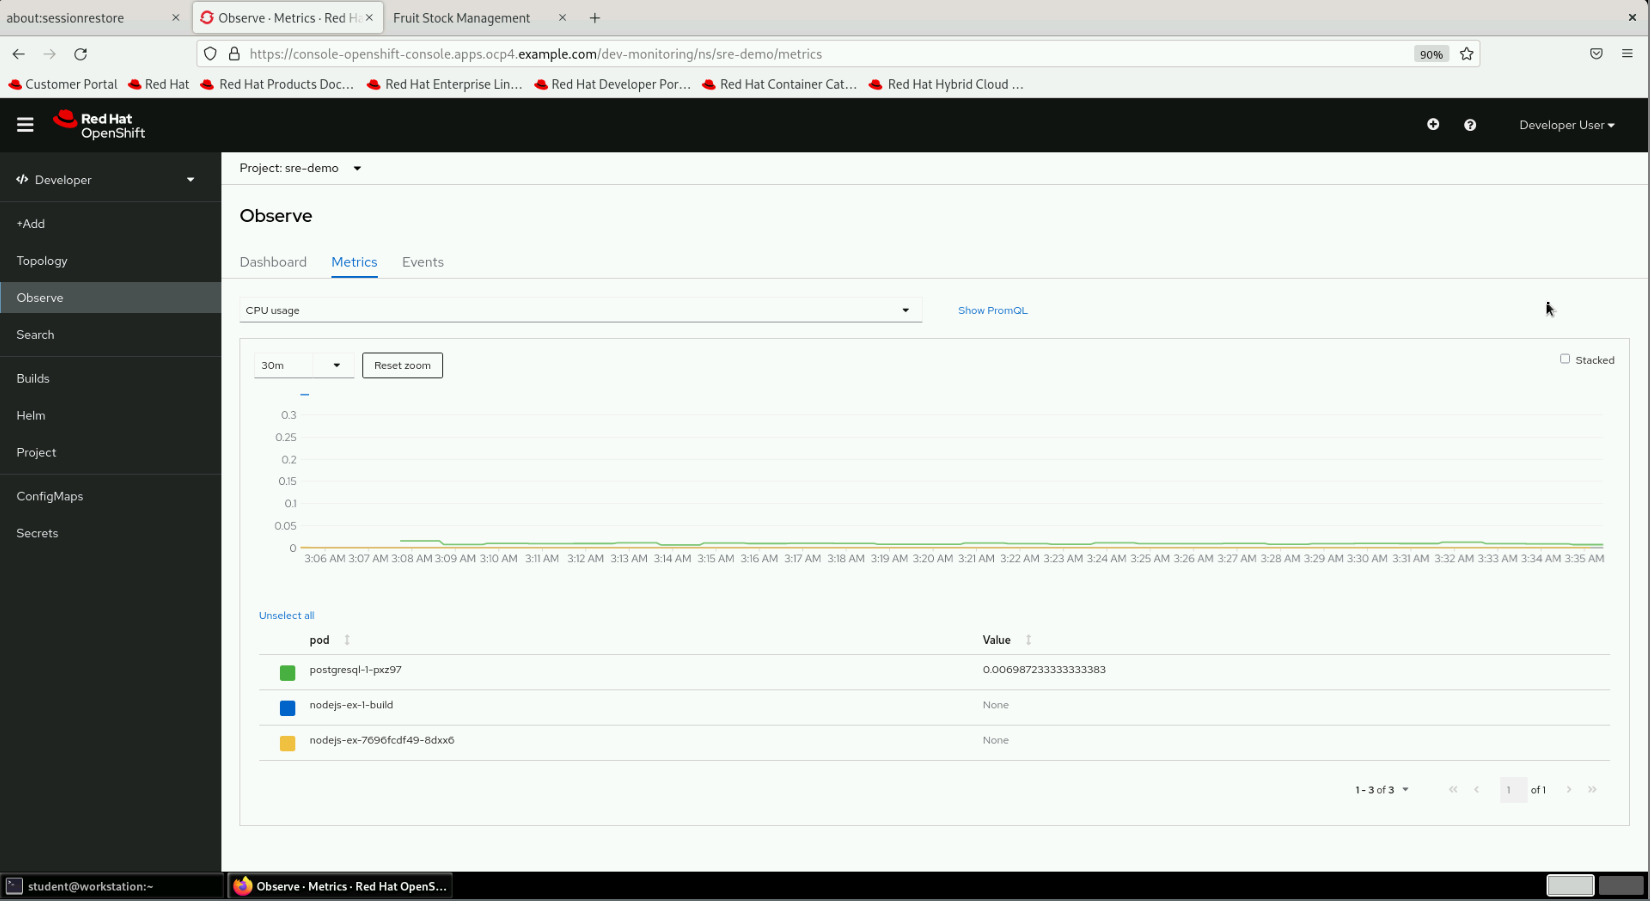
\includegraphics[width=1\linewidth]{imagenes/image20.png}
    \caption{Proceso de Source-to-Image (S2I)}
    \label{fig:openshift-ecosystem}
\end{figure}

\section{Fiabilidad, escalabilidad automática y auto-recuperación}

OpenShift incorpora características esenciales para garantizar la fiabilidad, la escalabilidad y la recuperación automática de las aplicaciones, principios fundamentales de SRE.

\subsection{Configuración de Probes (Sondas)}

Los probes (liveness y readiness) son esenciales para que OpenShift determine el estado de salud de una aplicación.  
Los probes de \textit{Liveness} le dicen a Kubernetes cuándo reiniciar un contenedor si este se ha quedado "colgado" o no responde. Esto asegura que los contenedores "muertos pero no caídos" sean reiniciados para intentar recuperarlos y mejorar la robustez de la aplicación.  
Los probes de \textit{Readiness} le dicen a Kubernetes cuándo un contenedor está listo para empezar a recibir tráfico, controlando cuándo puede recibir tráfico y garantizando que los usuarios siempre sean dirigidos a instancias que funcionan correctamente, evitando errores durante el inicio o problemas temporales.  
Ambas son evaluadas por el kubelet (agente principal que se ejecuta en cada nodo de OpenShift).

Se configuraron probes para el deployment del frontend:
\begin{verbatim}
oc set probe deployment/nodejs-ex \
  --liveness --get-url=http://:8080/ --initial-delay-seconds=15
oc set probe deployment/nodejs-ex \
  --readiness --get-url=http://:8080/ --initial-delay-seconds=5
\end{verbatim}

Con la configuración de estas sondas, el archivo YAML del deployment se habrá actualizado.


\subsection{Autoescalado}

Se habilitó el autoescalado horizontal para el deployment del frontend, de forma que OpenShift ajuste automáticamente el número de pods en función de la carga de CPU:
\begin{verbatim}
oc autoscale deployment/nodejs-ex --min=1 --max=3 --cpu-percent=50
\end{verbatim}

\begin{figure}[H]
    \centering
    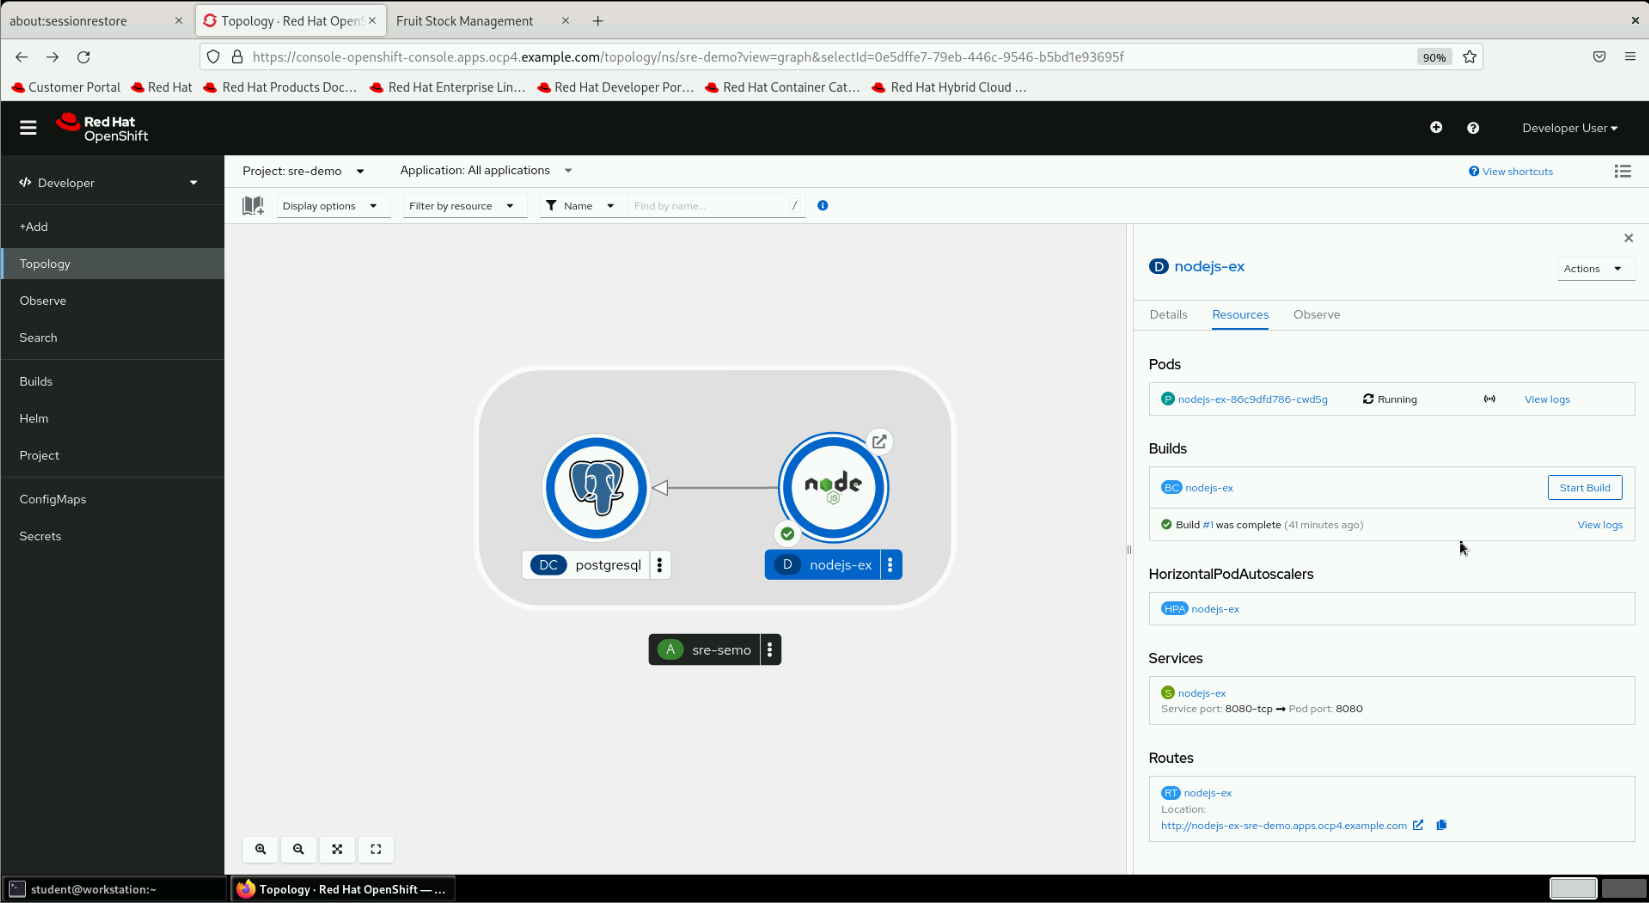
\includegraphics[width=0.8\linewidth]{imagenes/image155.png}
    \caption{Proceso de Source-to-Image (S2I)}
    \label{fig:openshift-ecosystem}
\end{figure}

Esto permite que la aplicación mantenga un rendimiento aceptable durante aumentos de demanda, sin necesidad de intervención humana.





\subsection{Recursos}

Se definieron límites y solicitudes de CPU y memoria para el deployment del frontend:
\begin{verbatim}
oc set resources deployment/nodejs-ex \
  --limits=cpu=500m,memory=512Mi \
  --requests=cpu=200m,memory=256Mi
\end{verbatim}

Esto asegura que los pods no consuman más recursos de los necesarios, y evita que un solo pod sobrecargue el nodo.

\subsection{Ejemplos prácticos de fiabilidad y recuperación}

Se llevaron a cabo una serie de pruebas para demostrar la fiabilidad inherente de OpenShift y su capacidad de auto-recuperación.

\subsubsection{Autoescalado en acción}

Para observar el comportamiento del autoescalado, se generó una carga sobre la aplicación utilizando un script que simula múltiples peticiones con ApacheBench (\texttt{ab}).  
Este es el script utilizado (\texttt{test-autoscaling.sh}):

\begin{verbatim}
#!/bin/bash

APP_URL="http://nodejs-ex-sre-demo.apps.ocp4.example.com/api/fruits"
TOTAL_REQUESTS=100000 # peticiones a enviar
CONCURRENCY=50        # peticiones simultaneas
DURATION=60           # tiempo (segundos)
echo "Iniciando ..."
echo "Duración: $DURATION segundos (puede variar)"
echo "Peticiones totales: $TOTAL_REQUESTS"
echo "Concurrencia: $CONCURRENCY"
echo "Generando carga sobre: $APP_URL"
echo "Observa con: oc get hpa -w && oc get pods -w"

# Comando ab
# -n: número de peticiones
# -c: número de peticiones concurrentes
# -t: tiempo máximo para el test (segundos) opcional podemos solo usar -n
# -k: habilita Keep-Alive HTTP (mejor rendimiento, más realista)
# -s: timeout (segundos)

ab -n $TOTAL_REQUESTS -c $CONCURRENCY -s 30 -k "$APP_URL"

echo "Test de carga con ab completado"
\end{verbatim}

Mientras la carga se generaba, se monitoreaba el estado del HPA (Horizontal Pod Autoscaler) y los pods en tiempo real para observar cómo OpenShift creaba automáticamente nuevas instancias para manejar el aumento de la demanda:
\begin{verbatim}
oc get hpa -w && oc get pods -w
\end{verbatim}

\begin{figure}[H]
    \centering
    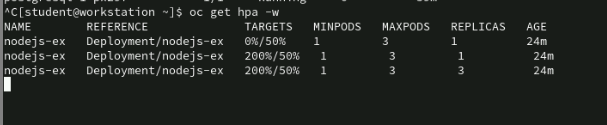
\includegraphics[width=1\linewidth]{imagenes/image27.png}
    \caption{Proceso de Source-to-Image (S2I)}
    \label{fig:openshift-ecosystem}
\end{figure}


Después de generar carga, el HPA mostró el aumento de pods hasta el máximo configurado (en este caso, 3 réplicas). ApacheBench mostró una carga significativa con \texttt{Requests per second: 2066.19 [\#/sec] (mean)} y \texttt{Time per request (mean): 24.196 [ms]}, lo que se resume en un pico de uso de CPU visible en los gráficos de monitoreo de OpenShift.

\begin{figure}[H]
    \centering
    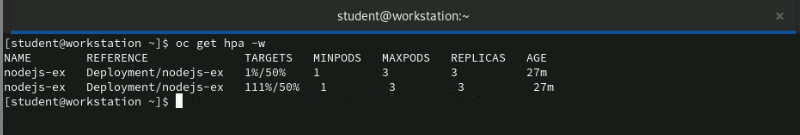
\includegraphics[width=1\linewidth]{imagenes/image7.png}
    \caption{Proceso de Source-to-Image (S2I)}
    \label{fig:openshift-ecosystem}
\end{figure}

\begin{figure}[H]
    \centering
    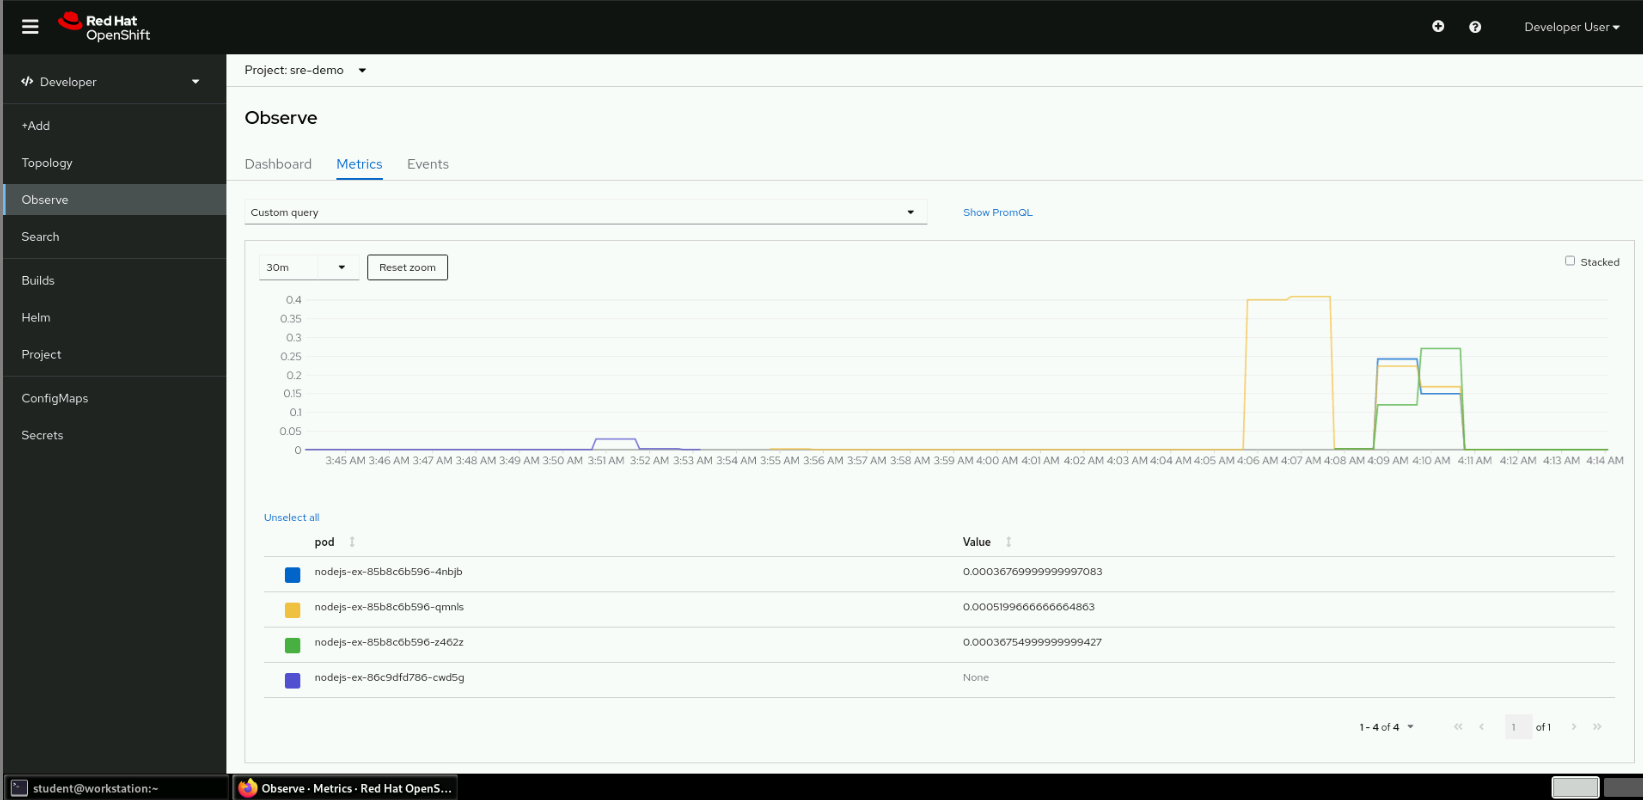
\includegraphics[width=0.95\linewidth]{imagenes/image5.png}
    \caption{Proceso de Source-to-Image (S2I)}
    \label{fig:openshift-ecosystem}
\end{figure}

\begin{figure}[H]
    \centering
    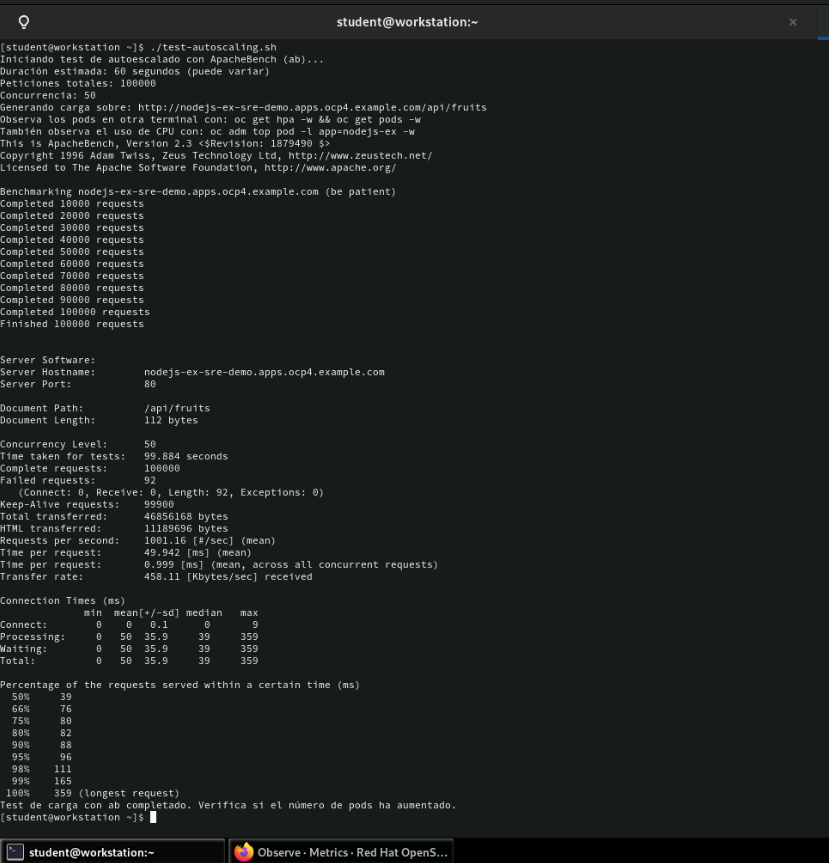
\includegraphics[width=1\linewidth]{imagenes/image144.png}
    \caption{Proceso de Source-to-Image (S2I)}
    \label{fig:openshift-ecosystem}
\end{figure}


Es importante notar que, incluso después de que la carga termine, las réplicas pueden tardar unos 5 minutos en desescalar completamente debido a la ventana de estabilización del HPA. Tras 5 minutos volverá a ser solo 1 pod.
\newpage

\begin{figure}[H]
    \centering
    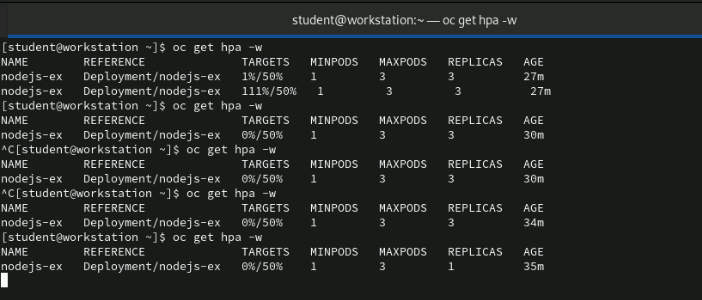
\includegraphics[width=1\linewidth]{imagenes/image1.png}
    \caption{Proceso de Source-to-Image (S2I)}
    \label{fig:openshift-ecosystem}
\end{figure}


\subsubsection{Auto-recuperación de pods}

Para demostrar la capacidad de auto-recuperación de la plataforma, se eliminó manualmente un pod de la aplicación:
\begin{verbatim}
oc delete pod $(oc get pod -l app=nodejs-ex -o name)
\end{verbatim}

OpenShift, al detectar el fallo y gracias a la configuración de sondas y réplicas, automáticamente creó un nuevo pod para reemplazar al eliminado, manteniendo así la disponibilidad del servicio sin intervención manual. Este comportamiento es posible gracias a las sondas y al deployment (siempre hay 1 como mínimo por defecto), así el sistema se recupera por sí mismo ante fallos comunes como borrar sin querer el pod.


\subsubsection{Comprobación de readiness/liveness}

Para entender cómo OpenShift reacciona a un pod que no funciona bien, se simuló un fallo en la sonda de readiness. Se cambió el puerto de la sonda de readiness a uno incorrecto (de 8080 a 9999), haciendo que la sonda falle y OpenShift marque ese pod como no listo para recibir tráfico.

Se monitorea el estado del pod en otra terminal:
\begin{verbatim}
oc get pods -w
\end{verbatim}

Luego, se ejecuta el comando para cambiar la sonda:
\begin{verbatim}
oc set probe deployment/nodejs-ex --readiness --get-url=http://:9999/ --initial-delay-seconds=5
\end{verbatim}

Tras ejecutar este comando, se observará que el pod se muestra como 0/1 Running en la columna READY. Esto significa que la sonda de readiness ha fallado para este pod, y OpenShift lo considera "no listo" para recibir tráfico.

\begin{figure}[H]
    \centering
    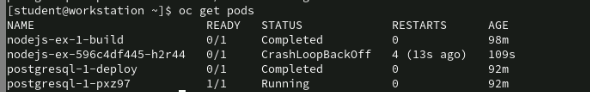
\includegraphics[width=1\linewidth]{imagenes/image16.png}
    \caption{Proceso de Source-to-Image (S2I)}
    \label{fig:openshift-ecosystem}
\end{figure}

Este resultado demuestra que la prueba de falla de readiness ha funcionado. Cuando un pod está 0/1 Ready, OpenShift lo saca del balanceador de carga. Esto significa que el tráfico se dirigirá a otros pods "listos" y, si este fuera el único pod, la aplicación sería inaccesible externamente, lo que confirma el problema inicial experimentado.

\begin{figure}[H]
    \centering
    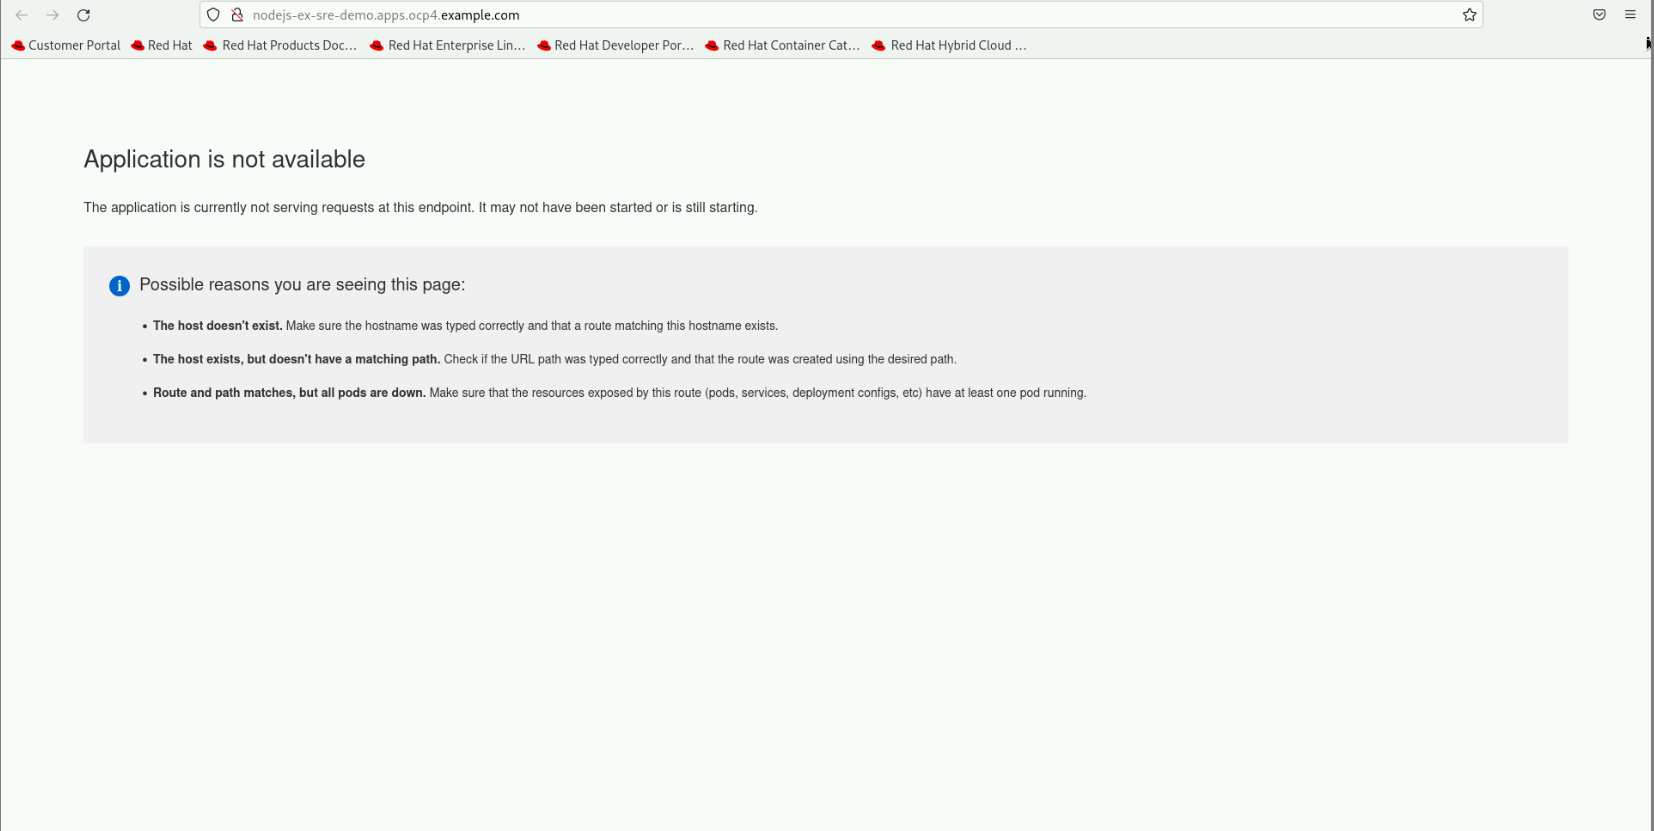
\includegraphics[width=1\linewidth]{imagenes/image6.png}
    \caption{Proceso de Source-to-Image (S2I)}
    \label{fig:openshift-ecosystem}
\end{figure}

\newpage

Posteriormente, se restauró la configuración correcta de la sonda para verificar la recuperación del estado "Ready" del pod:
\begin{verbatim}
oc set probe deployment/nodejs-ex --readiness --get-url=http://:8080/ --initial-delay-seconds=5
\end{verbatim}

\begin{figure}[H]
    \centering
    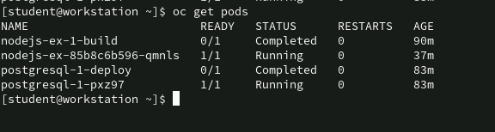
\includegraphics[width=1\linewidth]{imagenes/image177.png}
    \caption{Proceso de Source-to-Image (S2I)}
    \label{fig:openshift-ecosystem}
\end{figure}

Las sondas de Liveness se aseguran de que los contenedores "muertos pero no caídos" sean reiniciados para intentar recuperarlos, mejorando la robustez de la aplicación.  
Las sondas de Readiness controlan cuándo un contenedor puede recibir tráfico, garantizando que los usuarios siempre sean dirigidos a instancias que funcionan correctamente y evitando errores durante el inicio o problemas temporales.


\subsection{Actualización Automática de la Aplicación (CI/CD Básico)}

OpenShift facilita la implementación de un mecanismo de actualización continua cuando se realizan cambios en el repositorio de código fuente (git). Esto se logra configurando un trigger automático sobre el BuildConfig. Este comportamiento puede estar ya habilitado por defecto, pero se puede comprobar o forzar con:
\begin{verbatim}
oc set triggers bc/nodejs-ex --from-github=true --auto
\end{verbatim}

Además, en situaciones donde no se desea esperar a un push o se requiere forzar una construcción, se puede iniciar manualmente un nuevo build con el siguiente comando:
\begin{verbatim}
oc start-build nodejs-ex
\end{verbatim}

Este enfoque demuestra cómo se puede implementar un flujo básico de CI/CD (Continuous Integration/Continuous Deployment) directamente desde el control de versiones, agilizando el ciclo de entrega de software y reduciendo el esfuerzo manual.

\vspace{\baselineskip}

\newpage



